\documentclass[a4paper]{scrreprt}
\usepackage[ngerman]{babel}
\usepackage[T1]{fontenc}
\usepackage[utf8]{inputenc}
\usepackage{graphicx}
\graphicspath{ {./} }
\usepackage{makecell}
\usepackage[hidelinks]{hyperref} 
\title{Shop Stati}
\author{Michael Ritter <michael.ritter@cloudrexx.com>}

\begin{document}
    \selectlanguage{ngerman}
    \maketitle
    \tableofcontents
    \cleardoublepage
    \chapter{Stand dieser Dokumentation}
        Dies ist ein Draft. Die Aussagen basieren auf der aktuellen Version des
        Shops.
    \chapter{Bedeutungsübersicht der verfügbaren Stati}
        \section{Pendent}
        Die Bezahlung wurde noch nicht beendet, unterbrochen oder es trat ein
        unbekanntes Problem auf. Bei externen Zahlungsanbietern besteht in der
        Regel für den Kunden die Möglichkeit, den Zahlungsvorgang zu wiederholen.
        In diesem Fall wird eine neue Bestellung eingetragen und als ``Bestätigt''
        gekennzeichnet, sobald dies erfolgreich geschehen ist. Die Pendente
        Bestellung bleibt in der Datenbank und kann im Backend gelöscht werden.

        \section{Bestätigt}
        Der Bestellvorgang wurde erfolgreich abgeschlossen. Die Zahlung ist
        vorläufig abgeschlossen (Rechnung / Nachnahme). Die Ware wurde noch
        nicht versandt.

        \section{Gelöscht}
        Die Bestellung wurde manuell gelöscht.

        \section{Annuliert}
        Abbruch der Bestellung.

        \section{Abgeschlossen}
        Die Bezahlung ist erfolgt und die Ware wurde versandt.

        \section{Bezahlt}
        Die Bezahlung ist endgültig abgeschlossen, die Ware aber nicht versandt.

        \section{Versandt}
        Die Ware wurde versandt, die Bezahlung ist noch nicht erfolgt
        (Rechnung / Nachnahme).

    \chapter{Automatisch gesetzte Stati}
        Die folgende Tabelle zeigt auf, unter welchen Umständen eine Bestellung
        automatisch welchen Status erhält: \\ \\
        \resizebox{\textwidth}{!}{
            \begin{tabular}{|c||c|c|c|}
                \hline
                & Bezahlung abgeschlossen & Vertrieb abgeschlossen & Bemerkungen \\
                \hline\hline
                Pendent & - & - & Bezahlung unterbrochen oder fehlgeschlagen \\
                \hline
                Annuliert & - & - & Abbruch beim Zahlungsanbieter \\
                \hline
                Bestätigt & x\footnote{Bezahlung nur vorerst abgeschlossen!} & - & Interne Zahlungsmethode \\
                \hline
                Bezahlt & x & - & Online-Zahlung \\
                \hline
                Versandt & - & x & \makecell{Vertriebsart ``Download'' oder nach Versand \\ gegen Rechnung/Nachnahme} \\
                \hline
                Abgeschlossen & x & x & \makecell{Hiess früher ``Erledigt''. Online-Zahlung \\ mit Vertriebsart ``Download''.} \\
                \hline
            \end{tabular}
        }

    \chapter{Die Stati im Detail}
        \section{Pendent}
        Untenstehende Folgestati werden, abgesehen von ``Gelöscht'', im
        Normalfall vom System automatisch gesetzt. \\
        \resizebox{\textwidth}{!}{
            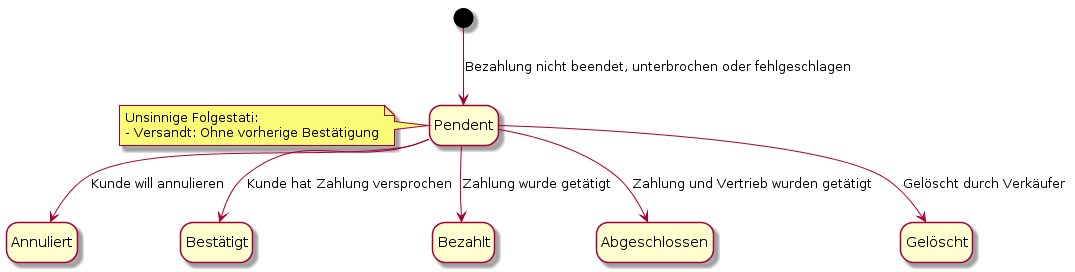
\includegraphics{Status.png}
        }

        \section{Bestätigt}
        \resizebox{\textwidth}{!}{
            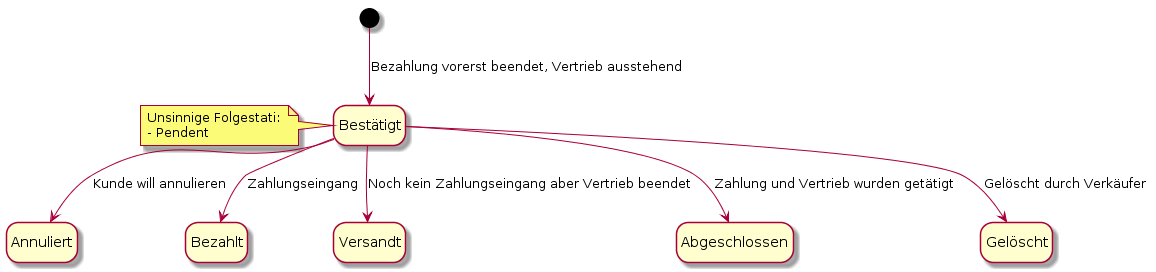
\includegraphics{Status_001.png}
        }

        \section{Gelöscht}
        \resizebox{\textwidth}{!}{
            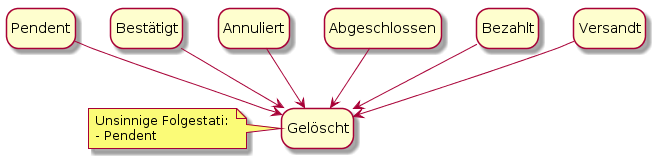
\includegraphics{Status_004.png}
        }

        \section{Annuliert}
        \resizebox{\textwidth}{!}{
            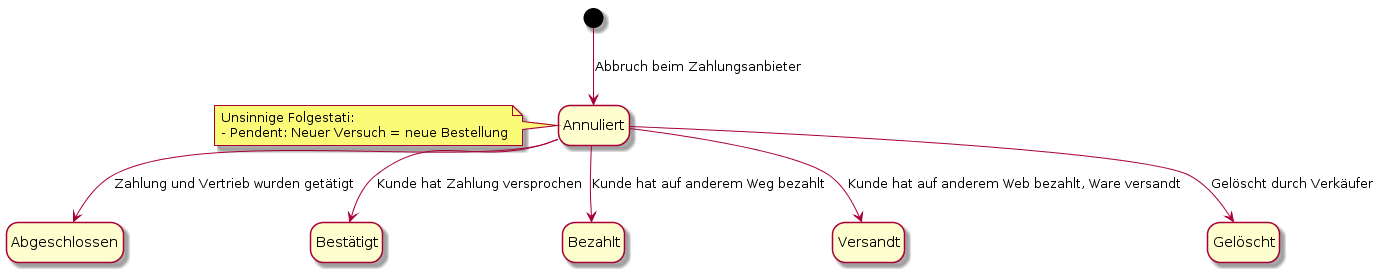
\includegraphics{Status_005.png}
        }

        \section{Abgeschlossen}
        Ein Folgestatus des Status ``Abgeschlossen'' ist nur zur Fehlerkorrektur
        sinnvoll (Bestellung wurde versehentlich auf ``Abgeschlossen'' gestellt). \\
        \resizebox{\textwidth}{!}{
            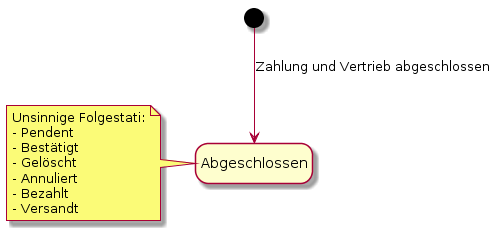
\includegraphics{Status_006.png}
        }

        \section{Bezahlt}
        \resizebox{\textwidth}{!}{
            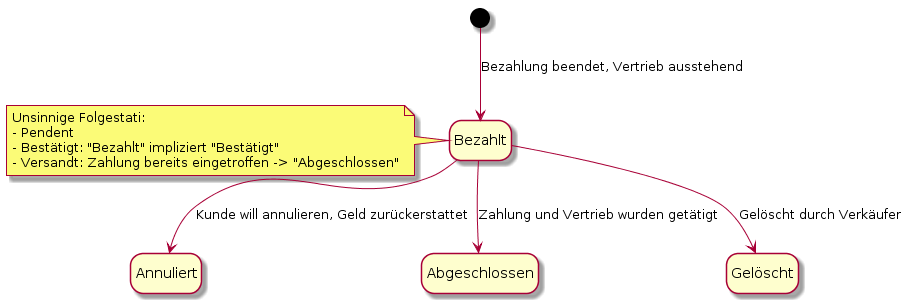
\includegraphics{Status_002.png}
        }

        \section{Versandt}
        \resizebox{\textwidth}{!}{
            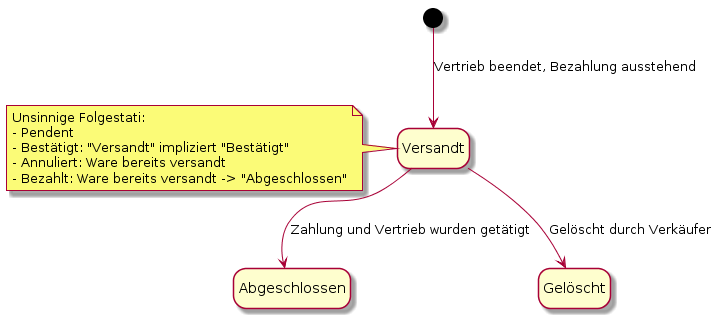
\includegraphics{Status_003.png}
        }
    \chapter{Mails}
        \section{Bestätigungsmail}
            Wenn das Bestätigungsmail ausgelöst wird, wird auch der Bestand angepasst.

            \subsection{Frontend: interne Zahlungsmethode}
            Shop::success() -> Orders::update\_status() -> ShopLibrary::sendConfirmationMail()
            -> Orders::getSubstitutionArray() -> Product::decreaseStock() \\ \\
            Dies wird nur beim Wechsel vom Status ``Pendent'' zu einem der Stati
            ``Bestätigt'', ``Bezahlt'', ``Versandt'' oder ``Abgeschlossen'' ausgelöst.

            \subsection{Frontend: externe Zahlungsmethode}
            Gleich wie interne Zahlungsmethode, nur wird die Methode success() erst
            asynchron vom Zahlungsanbieter aufgerufen.

            \subsection{Backend}
            Das Bestätigungsmail kann aus dem Backend nicht ausgelöst werden. Gem.
            Code wäre das zwar möglich, das Backend müsste aber \$\_GET['sendmail']
            als nicht leer übermitteln, was es nicht tut/kann.

        \section{Verarbeitung-abgeschlossen-Mail}
            Beim Wechsel zum Status ``Abgeschlossen'' im Backend wird, sofern
            der entsprechende Confirm-Dialog angenommen wurde, eine Mail
            ausgelöst. Dies hat keinen Einfluss auf den Bestand.

\end{document}
